\section{Results}
\label{sec:results}
Results from the combinatoric method and the closest-match method are statistically combined. Systematic uncertainties in the two methods are classified based on their correlation coefficients: those with a correlation coefficient greater than 0.1, such as uncertainties from simulation statistics, cluster ADC and $\phi$-size selections, machine and detector stability, model dependence, and secondary contributions, are treated as fully correlated. In contrast, uncertainties with a correlation coefficient below 0.1, such as those arising from tracklet reconstruction criteria, are considered uncorrelated. 
The weighted average of the two approaches, $\bar{X}$, and the uncorrelated uncertainty on the weighted average result, $\sigma_X$, are computed as:  
\begin{equation}
\begin{split}
\bar{X} \pm \sigma_X & = \frac{ w_{\text{Comb.}} X_{\text{Comb.}} + w_{\text{C.-m.}} X_{\text{C.-m.}}}{w_{\text{Comb.}} + w_{\text{C.-m.}}} \pm \left(w_{\text{Comb.}} + w_{\text{C.-m.}} \right)^{-1/2}, \\ 
 w_{\text{Comb.}} & = \frac{1}{(\sigma_{X,\text{Comb.}})^2}\quad \text{,}\quad w_{\text{C.-m.}} = \frac{1}{(\sigma_{X,\text{C.-m.}})^2}, \\
\end{split}
\label{eq:weiavg-uncorrunc}
\end{equation}

where \(X_\text{Comb./C.-m.}\), \(\sigma_{X,\text{Comb./C.-m.}}\), and $w_{\text{Comb./C.-m.}}$ represent the value, uncorrelated uncertainty, and the weight reported by the two methods. The weights vary with centrality and pseudorapidity, with an average weight ratio of $w_{\text{C.-m.}} / (w_{\text{Comb.}} + w_{\text{C.-m.}})$ = 0.83.
The correlated uncertainty on the weighted average result, $\bar{s}$, is calculated:  
\begin{equation}
\bar{s} = \sqrt{\sum_k \bigg[\frac{w_{\text{Comb.}}}{w_{\text{Comb.}}+w_{\text{C.-m.}}}(s_{\text{Comb.}})_k + \frac{w_{\text{C.-m.}}}{w_{\text{Comb.}}+w_{\text{C.-m.}}}(s_{\text{C.-m.}})_k\bigg]^2},
\label{eq:corrunc}
\end{equation}
where $(s_{\text{Comb.}})_{k}$ and $(s_{\text{C.-m.}})_{k}$ denote the uncertainties from the combinatoric method and the closest-match method (indexed by $k$), respectively. The total uncertainty of the weighted average result is obtained by:  
\begin{math}
\sigma_{\text{total}} = \sqrt{\bar{s}^2 + \sigma_X^2}.
\end{math} 

The combination strategy used in this measurement closely follows procedures outlined by the Particle Data Group and the \cms experiment~\cite{ParticleDataGroup:2024cfk, CMS:2011aqh}, specifically to account for dominant correlated uncertainties in the two analysis methods, where Equations~\ref{eq:weiavg-uncorrunc} and \ref{eq:corrunc} are applicable. Notably, the combined uncertainty has a modest increase compared to the method with the smaller uncertainty in some instances. In contrast, the use of a best limit unbiased estimator~\cite{5f88760e-8167-31ed-9022-4d8c4dafd76a} is seen to decrease the overall uncertainty but cause the central value of some bins to fall outside the mean values defined by the individual methods. The approach adopted in this paper may not be universally applicable, and careful consideration is required when extending it to other measurements with different correlation structures.

Figure~\ref{fig:dndeta-allcent} presents \dndeta as a function of $\eta$ for various centrality intervals, showing results from both approaches as well as the combined result compared with measurements from \phobos~\cite{PHOBOS:2010eyu}. The results from both approaches are consistent within their respective uncertainties, which are obtained by summing all sources in quadrature under the assumption that individual uncertainties are independent and uncorrelated. The combined result remains in agreement with the \phobos measurements across the $\eta$ range covered in this analysis, with uncertainties in the \sphenix measurement calculated using the procedure described above.

The left panel of Figure~\ref{fig:dndeta-eta0avgnpart} presents \dndeta at mid-rapidity, averaged over $|\eta|<0.3$, as a function of centrality class, demonstrating that charged hadron multiplicity increases with collision centrality. The charged hadron density for the most central 3\% of events (0–3\% centrality bin) is measured to be $\dndeta|_{|\eta| < 0.3} = 723.4 \pm 45.3$.
Results from this analysis (black solid circles), obtained by combining two analysis methods as described above, are compared with previous RHIC measurements, including \phobos (blue open squares), \phenix (cyan open diamonds), and \brahms (purple open crosses). The shaded color bands represent the full systematic uncertainty. The \sphenix results are consistent with those from \phobos, \phenix, and \brahms within uncertainties across all centrality intervals. 

\begin{figure}[H]
  \centering
  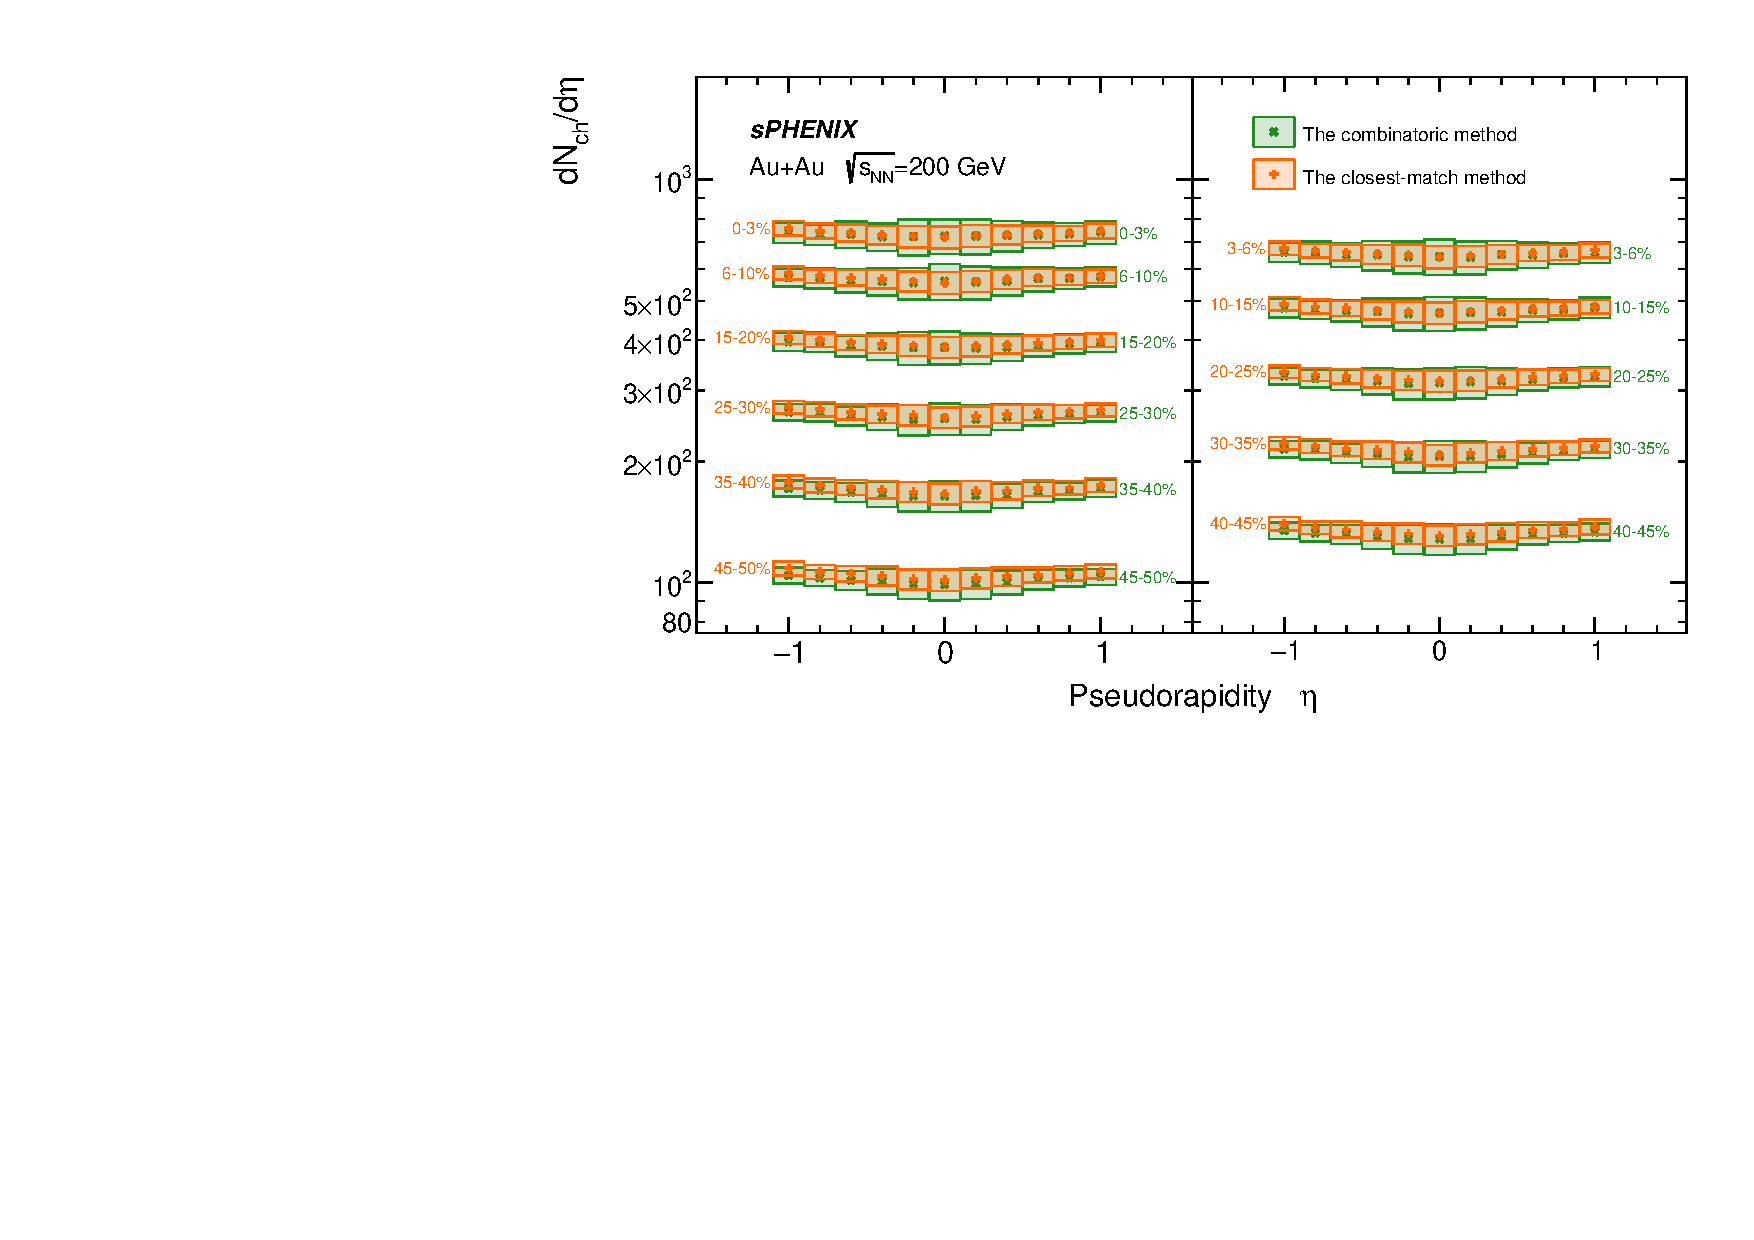
\includegraphics[width=0.85\textwidth]{fig/Results/dNdEta_RHIC_woBRAHMS_altCent.pdf}\\
  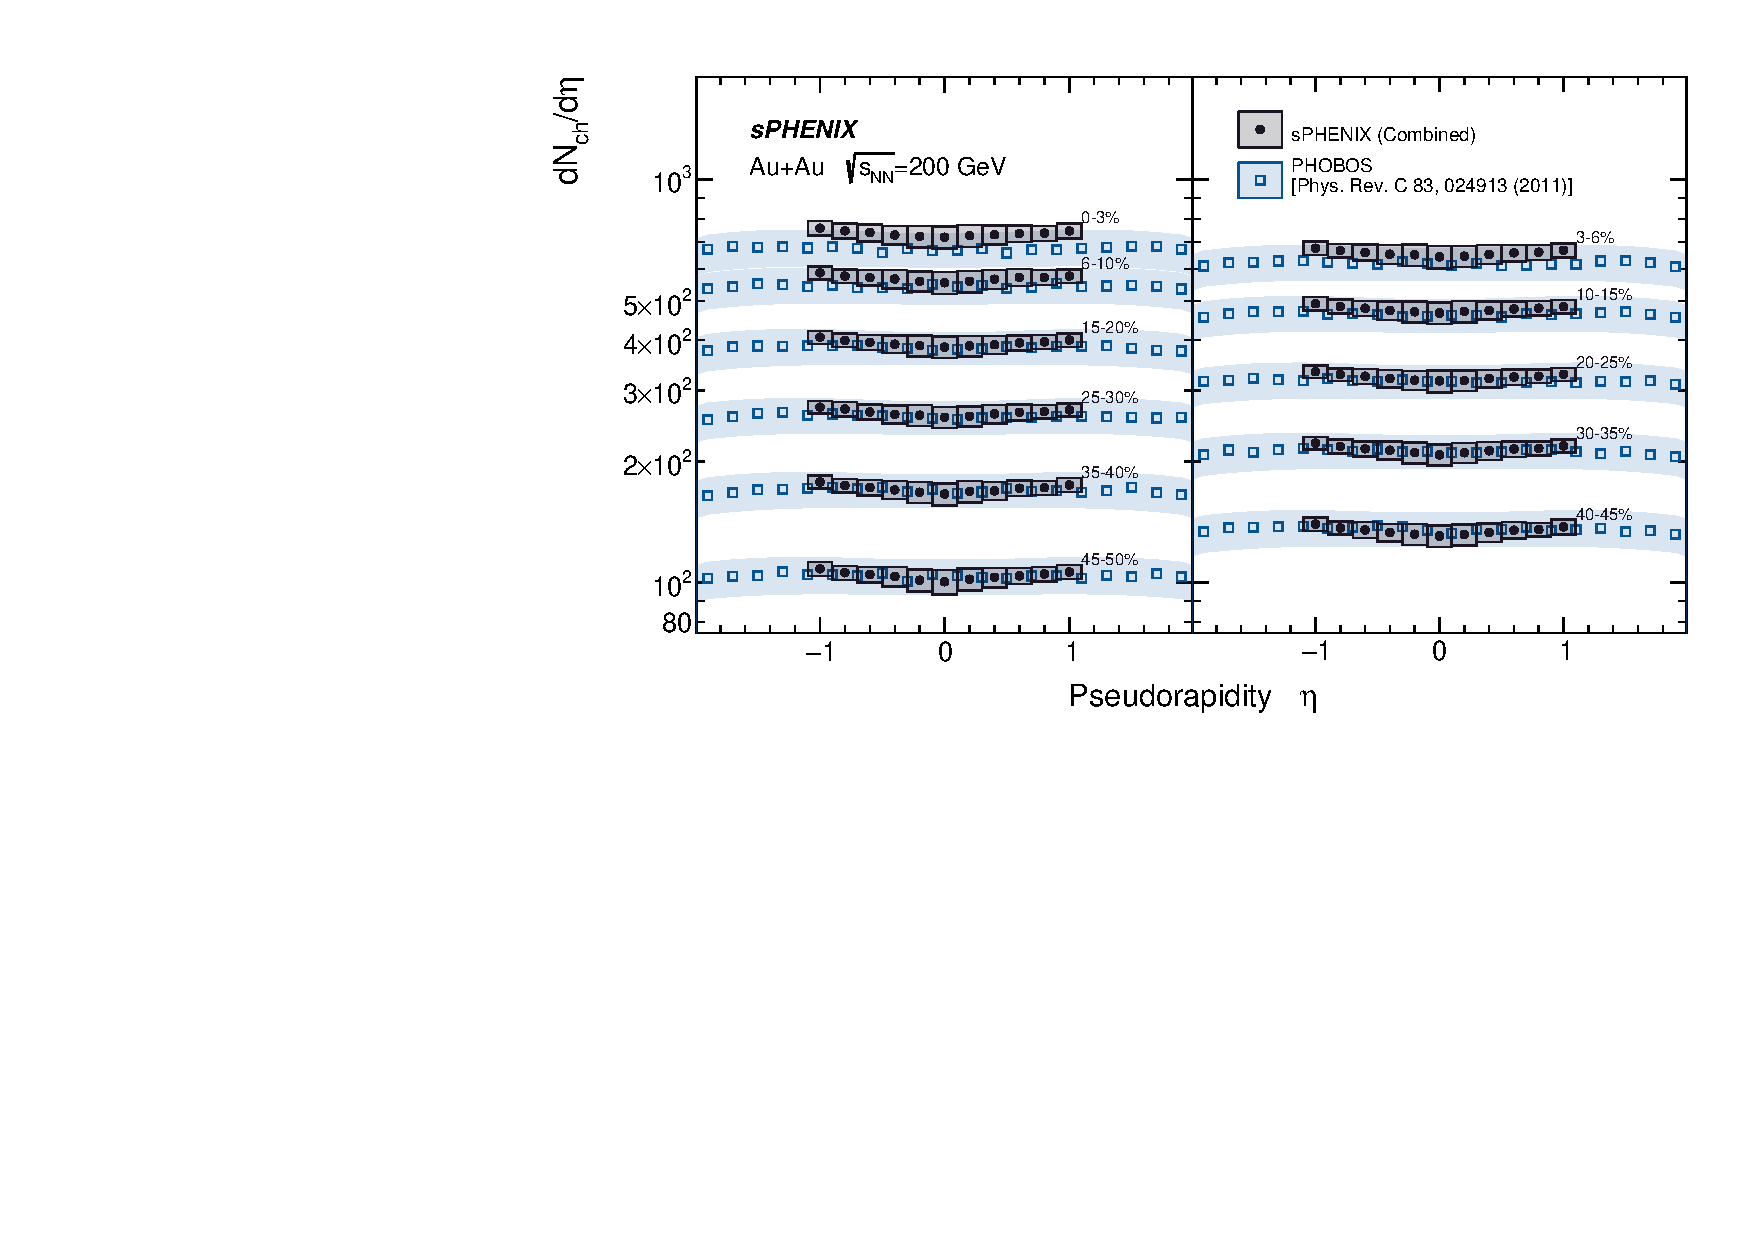
\includegraphics[width=0.85\textwidth]{fig/Results/dNdEta_RHIC_combine_woBRAHMS_altCent.pdf}
  \caption{Top: corrected \dndeta measurements from the combinatoric method (green solid crosses and green transparent filled boxes) and the closest-match method (orange solid pluses and transparent filled boxes) as a function of $\eta$ over the measurement range $|\eta|<1.1$, spanning from 0–3\% central to 45–50\% mid-central \auau events. The vertical extent of each box represents the total systematic uncertainty for each analysis method, obtained by summing all sources in quadrature under the assumption that individual uncertainty sources are independent and uncorrelated. Bottom: \dndeta measurements from the combination of both analysis methods (black solid circles and transparent filled boxes) as a function of $\eta$ over the range $|\eta|<1.1$, covering centralities from 0–3\% to 45–50\% in \auau collisions. The vertical size of each box represents the full combined uncertainty, calculated using the procedure outlined above. For comparison, \phobos measurements in the same centrality classes are shown as blue open squares~\cite{PHOBOS:2010eyu}, with the filled area representing the total uncertainty.} 
  \label{fig:dndeta-allcent}
\end{figure}

The right panel of Figure~\ref{fig:dndeta-eta0avgnpart} presents the average \dndeta per participant pair, $N_{\text{part}}/2$, as a function of $\langle N_{\text{part}}\rangle$, to evaluate the relationship between particle production and the number of participating nucleons. The \sphenix data exhibit the characteristic non-linear increase, with a steeper rise in more peripheral collisions compared to central collisions. The measured $\dndeta|_{|\eta|<0.3}/(N_{\text{part}}/2$) values range from approximately $2.4$ to $4.0$ charged hadrons per participant pair on average, over the \npart range covered in this analysis.
The \sphenix results are consistent with those from \phobos, \phenix, and \brahms within uncertainties across all centrality bins considered. This observable is further compared to predictions from the \hijing, \epos, and \ampt MC heavy-ion event generators, with results indicating that the \sphenix measurement is most compatible with \hijing in both magnitude and \npart dependence. 

\begin{figure}[t!]
  \centering
  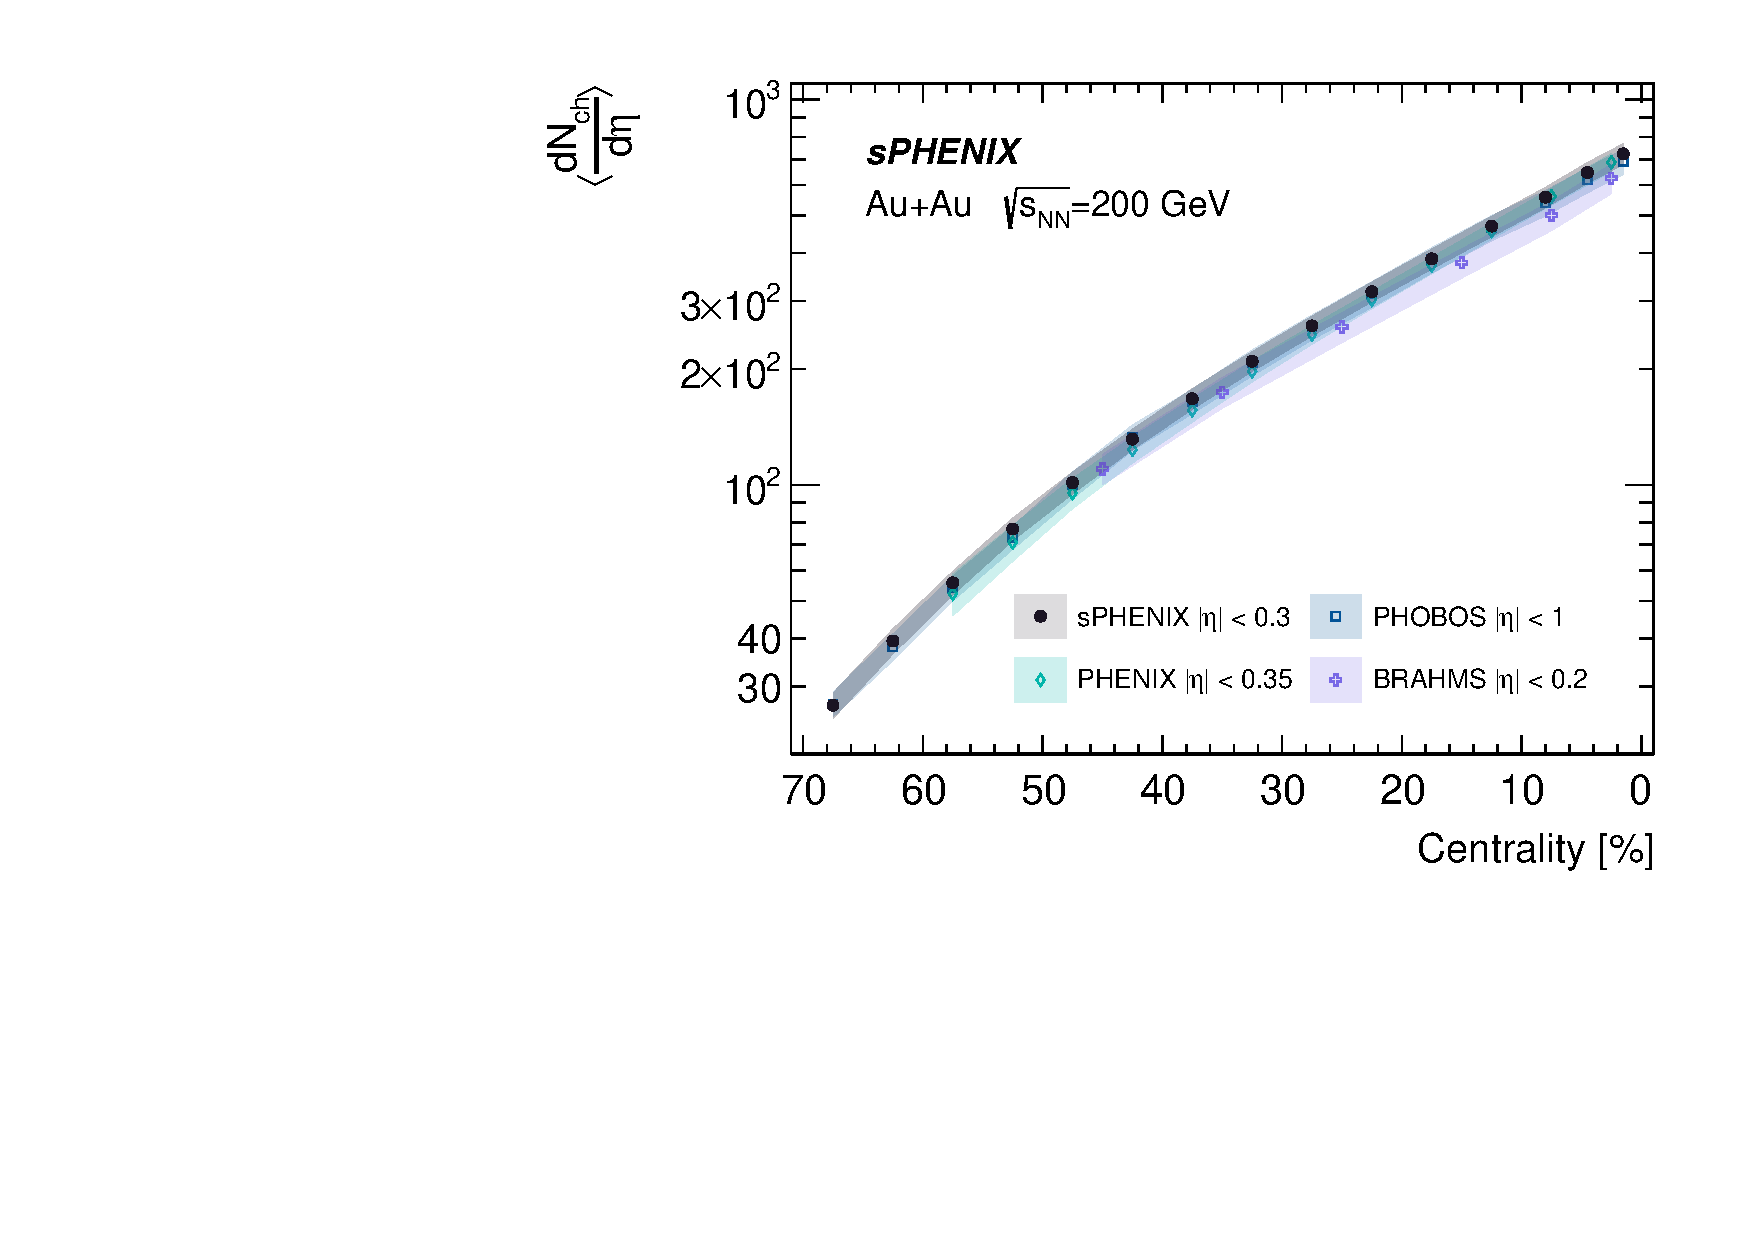
\includegraphics[width=0.5\textwidth]{fig/Results/dNdEta_eta0_RHIC_combine.pdf}~
  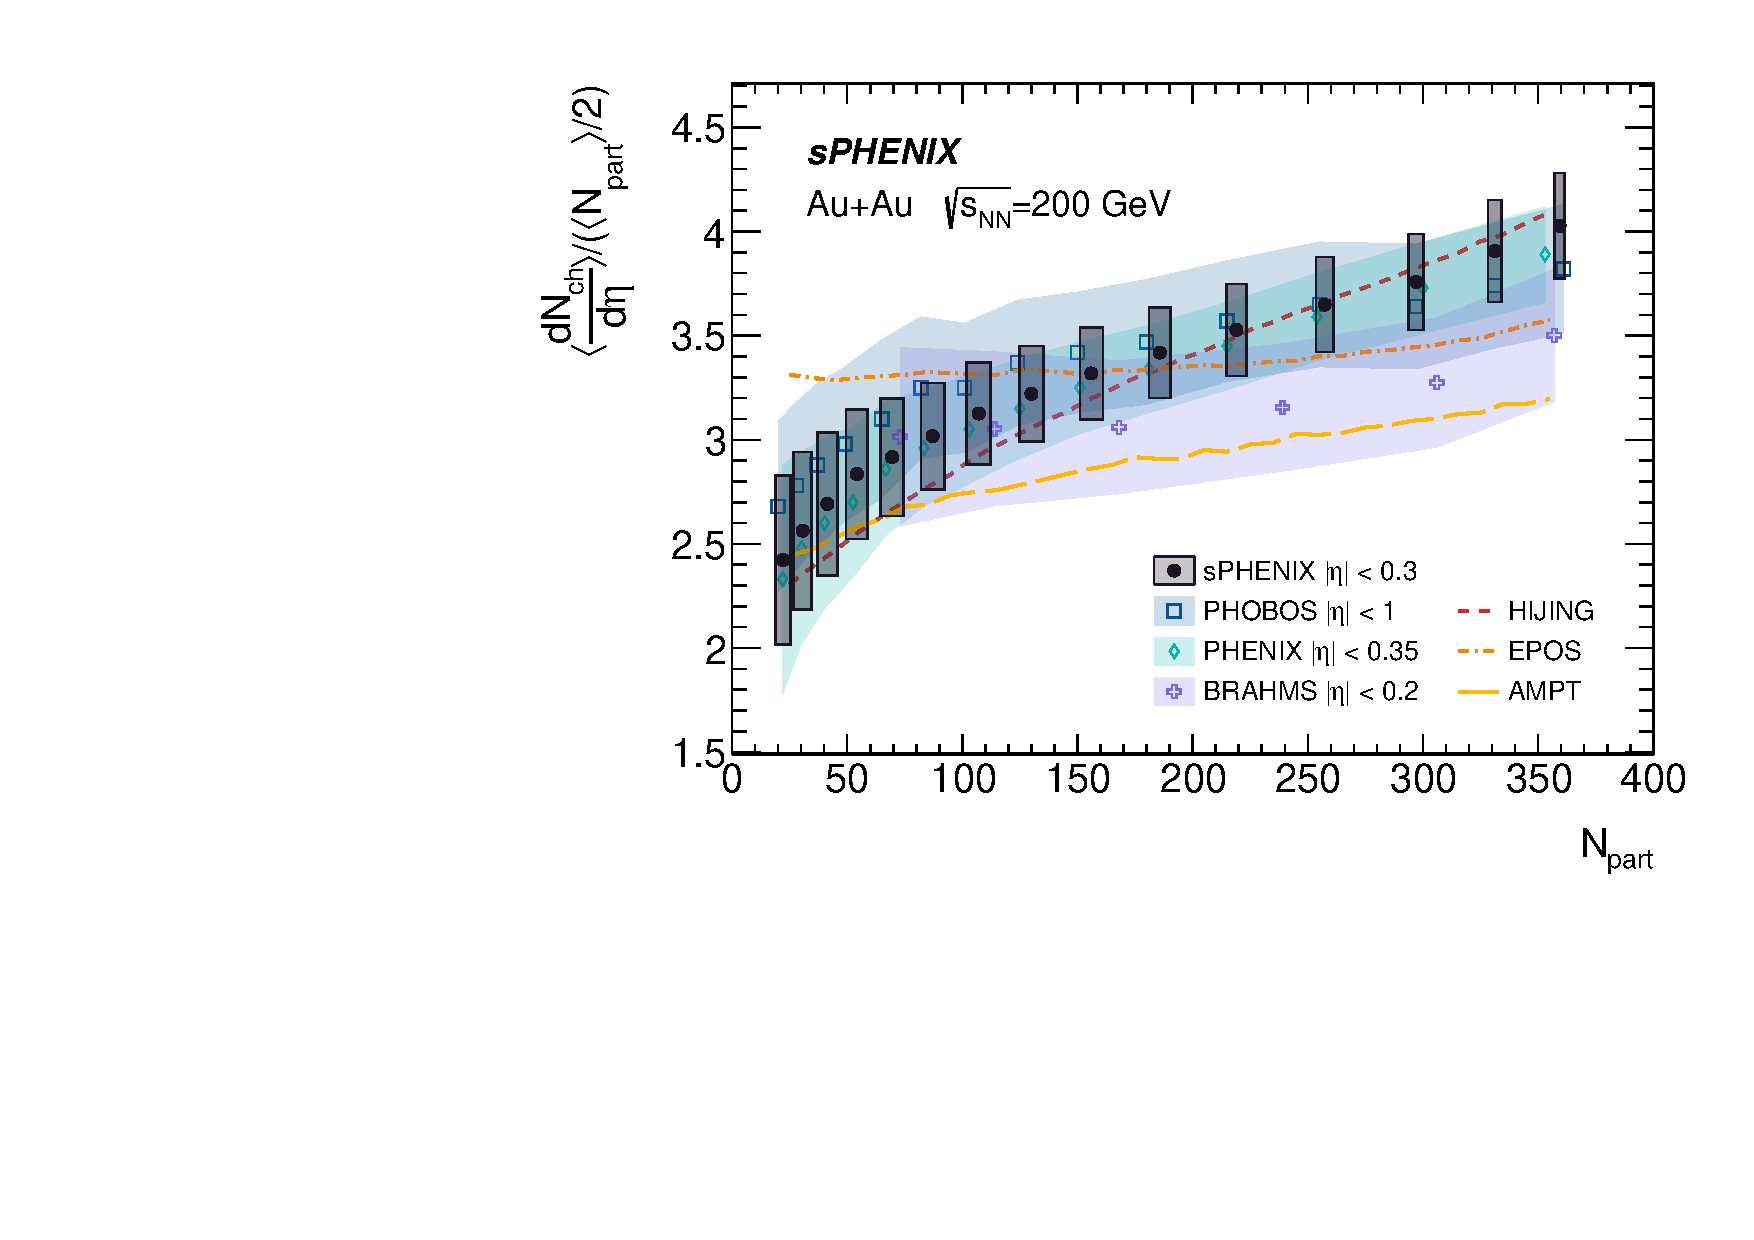
\includegraphics[width=0.5\textwidth]{fig/Results/dNdEta_eta0_divnpart2_RHIC_combine_style1.pdf}
  \caption{The \sphenix results are shown as black solid circles with transparent filled band/boxes indicating total uncertainties, while data from \phobos (blue open squares)~\cite{PHOBOS:2010eyu}, \phenix (cyan open diamonds)~\cite{PHENIX:2004vdg}, and \brahms (purple open crosses)~\cite{BRAHMS:2001llo} are presented for comparison. The colored bands represent the total systematic uncertainty for each presented measurement. Left: \sphenix combined \dndeta at mid-rapidity, averaged over \(|\eta| < 0.3\), as a function of event centrality. Right: the average \dndeta at mid-rapidity, normalised by the number of participant pairs, as a function of the number of participating nucleons.}
  \label{fig:dndeta-eta0avgnpart}
\end{figure}

The midrapidity charged hadron multiplicities, the number of participants, and the charged hadron multiplicities normalised to the number of participant pairs, $\langle$\npart$\rangle/2$, are summarized in Table~\ref{tab:results}. 

\begin{table}[t!]
    \centering
    \caption{Summary of the midrapidity charged hadron multiplicities, the number of participants, and the charged hadron multiplicities normalised to the number of participant pairs $\langle$\npart$\rangle/2$.}
    \onehalfspacing
    \begin{tabular}{c c c c}
        \toprule[1pt]
        \textbf{Bin} & \textbf{$\frac{dN_{\text{ch}}}{d\eta}\big|_{|\eta|<0.3}$} & $\langle$\textbf{\npart}$\rangle$ & $\frac{\dndeta|_{|\eta|<0.3}}{\langle N_{\text{part}}\rangle/2}$ \\
        \midrule[1pt]
        0\%-3\% & $723.4\pm45.3$ & $359.3\pm2.1$ & $4.0\pm0.3$ \\
        3\%-6\% & $646.9\pm40.2$ & $331.2\pm2.9$ & $3.9\pm0.2$ \\
        6\%-10\% & $558.1\pm33.7$ & $297.0\pm3.2$ & $3.8\pm0.2$ \\
        10\%-15\% & $469.5\pm28.5$ & $257.3\pm3.8$ & $3.6\pm0.2$ \\
        15\%-20\% & $386.3\pm23.0$ & $219.0\pm4.3$ & $3.5\pm0.2$ \\
        20\%-25\% & $317.4\pm18.6$ & $185.7\pm4.6$ & $3.4\pm0.2$ \\
        25\%-30\% & $258.9\pm15.2$ & $156.0\pm5.0$ & $3.3\pm0.2$ \\
        30\%-35\% & $209.3\pm12.3$ & $130.0\pm5.2$ & $3.2\pm0.2$ \\
        35\%-40\% & $167.4\pm10.2$ & $107.1\pm5.2$ & $3.1\pm0.2$ \\
        40\%-45\% & $131.4\pm8.0$ & $87.1\pm5.1$ & $3.0\pm0.3$ \\
        45\%-50\% & $101.3\pm6.6$ & $69.5\pm5.0$ & $2.9\pm0.3$ \\
        50\%-55\% & $76.8\pm5.2$ & $54.2\pm4.7$ & $2.8\pm0.3$ \\
        55\%-60\% & $55.7\pm3.9$ & $41.4\pm4.4$ & $2.7\pm0.3$ \\
        60\%-65\% & $39.3\pm2.9$ & $30.7\pm3.9$ & $2.6\pm0.4$ \\
        65\%-70\% & $26.8\pm2.0$ & $22.1\pm3.3$ & $2.4\pm0.4$ \\
        \bottomrule[1pt]
    \end{tabular}
    \label{tab:results}
\end{table}